\documentclass{ximera}

\input{../preamble.tex}

\outcome{Understand the Squeeze Theorem and how it can be used to find limit values.}
\outcome{Calculate limits using the Squeeze Theorem.}

\title[Dig-In:]{The Squeeze Theorem}

\begin{document}
\begin{abstract}
The Squeeze theorem allows us to exchange difficult functions for easy functions.
\end{abstract}
\maketitle

In mathematics, sometimes we can study complex functions by exchanging
them for simplier functions. The \textit{Squeeze Theorem} tells us one
situation where this is possible.

\begin{theorem}[Squeeze Theorem]\index{Squeeze Theorem}
  Suppose that
  \[
  g(x) \le f(x) \le h(x)
  \]
  for all $x$ close to $a$ but not necessarily equal to $a$. If
  \[
  \displaystyle\lim_{x\to a} g(x) = L = \lim_{x\to a} h(x),
  \] 
  then $\displaystyle\lim_{x\to a} f(x) = L$.
\end{theorem}

\begin{question}
  I'm thinking of a function $f$. I know that for all $x$
  \[
  0 \le f(x) \le x^2.
  \]
  What is $\displaystyle\lim_{x\to 0} f(x)$?
  \begin{multipleChoice}
    \choice{$f(x)$}
    \choice{$f(0)$}
    \choice[correct]{$0$}
    \choice{impossible to say}
  \end{multipleChoice}
\end{question}



\begin{example}
Consider the function
\[
f(x) = 
\begin{cases}
\sqrt[5]{x}\sin\left(\frac{1}{x}\right) & \text{if $x \ne 0$,}\\
0 & \text{if $x = 0$,}
\end{cases}
\]
\begin{image}
\begin{tikzpicture}
	\begin{axis}[
            domain=-.2:.2,    
            samples=500,
            width=6in,
            height=3in,
            axis lines =middle, xlabel=$x$, ylabel=$y$,
            yticklabels = {}, 
            every axis y label/.style={at=(current axis.above origin),anchor=south},
            every axis x label/.style={at=(current axis.right of origin),anchor=west},
            clip=false,
          ]
	  \addplot [very thick, penColor, smooth, domain=(-.2:-.02)] {abs(x)^(1/5)*sin(deg(1/x))};
          \addplot [very thick, penColor, smooth, domain=(.02:.2)] {x^(1/5)*sin(deg(1/x))};
	  \addplot [color=penColor, fill=penColor, very thick, smooth,domain=(-.02:.02)] {abs(x)^(1/5)} \closedcycle;
          \addplot [color=penColor, fill=penColor, very thick, smooth,domain=(-.02:.02)] {-abs(x)^(1/5)} \closedcycle;
        \end{axis}
\end{tikzpicture}
%% \caption[A continuous function.]{A plot of
%% \[
%% f(x)=
%% \begin{cases}
%% \sqrt[5]{x}\sin\left(\frac{1}{x}\right) & \text{if $x \ne 0$,}\\
%%  0 & \text{if $x = 0$.}
%% \end{cases}
%% \]
%% }
\end{image}
Is this function continuous at $x=0$?
\begin{explanation}
We must show that $\lim_{x\to 0} f(x) = \answer[given]{0}$. Note
\[
-|\sqrt[5]{x}|\le f(x) \le |\sqrt[5]{x}|.
\]
Since
\[
\lim_{x\to 0} -|\sqrt[5]{x}| = \answer[given]{0} = \lim_{x\to 0}|\sqrt[5]{x}|,
\]
we see by the Squeeze Theorem, Theorem, that
$\displaystyle\lim_{x\to 0} f(x) = \answer[given]{0}$. Hence $f(x)$ is continuous.

Here we see how the informal definition of continuity being that you
can ``draw it'' without ``lifting your pencil'' differs from the
formal definition.
\end{explanation}
\end{example}




\begin{example}
Compute:
\[
\displaystyle\lim_{\theta\to 0} \frac{\sin(\theta)}{\theta}
\]
\begin{explanation}
To compute this limit, use the Squeeze Theorem. First note that we
only need to examine $\theta\in \left(\frac{-\pi}{2}, \frac{\pi}{2}\right)$
and for the present time, we'll assume that $\theta$ is positive. Consider
the diagrams below:

\begin{image}
\begin{tabular}{ccc}
\begin{tikzpicture}
	\begin{axis}[
            xmin=-.1,xmax=1.1,ymin=-.1,ymax=1.1,
            axis lines=center,
            ticks=none,
            unit vector ratio*=1 1 1,
            xlabel=$x$, ylabel=$y$,
            every axis y label/.style={at=(current axis.above origin),anchor=south},
            every axis x label/.style={at=(current axis.right of origin),anchor=west},
          ]        
          \addplot [very thick, penColor2, smooth, domain=(-.2:.2+pi/2)] ({cos(deg(x))},{sin(deg(x))});
          \addplot [textColor] plot coordinates {(0,0) (1,.839)}; %% 40 degrees
          \addplot [very thick, penColor] plot coordinates {(.766,0) (.766,.643)}; %% 40 degrees
          \addplot [textColor] plot coordinates {(1,0) (1,.839)}; %% 40 degrees
          \addplot [very thick,penColor,fill=fill1] plot coordinates {(0,0) (.766,.643)}\closedcycle; %% triangle
          \addplot [textColor,smooth, domain=(0:40)] ({.15*cos(x)},{.15*sin(x)});
          \node at (axis cs:.15,.07) [anchor=west] {$\theta$};
          \node at (axis cs:.766,.322) [anchor=east] {$\sin(\theta)$};
          \node at (axis cs:.383,0) [anchor=north] {$\cos(\theta)$};
        \end{axis}
\end{tikzpicture} & 
\begin{tikzpicture}
	\begin{axis}[
            xmin=-.1,xmax=1.1,ymin=-.1,ymax=1.1,
            axis lines=center,
            ticks=none,
            unit vector ratio*=1 1 1,
            xlabel=$x$, ylabel=$y$,
            every axis y label/.style={at=(current axis.above origin),anchor=south},
            every axis x label/.style={at=(current axis.right of origin),anchor=west},
          ]        
          \addplot [draw=none,fill=fill1] plot coordinates {(0,0) (.766,.643)}\closedcycle; %% sector
          \addplot [draw=none, fill=fill1, samples=100, domain=(0:40)] ({cos(x)},{sin(x)})\closedcycle; %% sector 
          \addplot [very thick, penColor2, smooth, domain=(-.2:.2+pi/2)] ({cos(deg(x))},{sin(deg(x))});
          \addplot [textColor] plot coordinates {(0,0) (1,.839)}; %% 40 degrees
          \addplot [textColor] plot coordinates {(.766,0) (.766,.643)}; %% 40 degrees
          \addplot [textColor] plot coordinates {(1,0) (1,.839)}; %% 40 degrees          
          \addplot [textColor,smooth, domain=(0:40)] ({.15*cos(x)},{.15*sin(x)});
          \addplot [very thick,penColor] plot coordinates {(0,0) (.766,.643)}; %% sector
          \addplot [very thick,penColor] plot coordinates {(0,0) (1,0)}; %% sector
          \addplot [very thick, penColor, smooth, domain=(0:40)] ({cos(x)},{sin(x)}); %% sector
          \node at (axis cs:.15,.07) [anchor=west] {$\theta$};
          \node at (axis cs:.5,0) [anchor=north] {$1$};
        \end{axis}
\end{tikzpicture} & 
\begin{tikzpicture}
	\begin{axis}[clip=false,
            xmin=-.1,xmax=1.1,ymin=-.1,ymax=1.1,
            axis lines=center,
            ticks=none,
            unit vector ratio*=1 1 1,
            xlabel=$x$, ylabel=$y$,
            every axis y label/.style={at=(current axis.above origin),anchor=south},
            every axis x label/.style={at=(current axis.right of origin),anchor=west},
          ]        
          \addplot [very thick,penColor,fill=fill1] plot coordinates {(0,0) (1,.839)}\closedcycle; %% triangle          
          \addplot [very thick, penColor2, smooth, domain=(-.1:1.671)] ({cos(deg(x))},{sin(deg(x))});
          \addplot [very thick, penColor] plot coordinates {(0,0) (1,.839)}; %% 40 degrees
          \addplot [textColor] plot coordinates {(.766,0) (.766,.643)}; %% 40 degrees
          \addplot [very thick, penColor] plot coordinates {(1,0) (1,.839)}; %% 40 degrees          
          \addplot [textColor,smooth, domain=(0:40)] ({.15*cos(x)},{.15*sin(x)});
          \node at (axis cs:.15,.07) [anchor=west] {$\theta$};
          \node at (axis cs:.5,0) [anchor=north] {$1$};
          \node at (axis cs:1,.42) [anchor=west] {$\tan(\theta)$};
        \end{axis}
\end{tikzpicture}\\
Triangle $A$ & Sector & Triangle $B$ \\
\end{tabular}
\end{image}


From our diagrams above we see that
\[
\text{Area of Triangle $A$} \le \text{Area of Sector} \le \text{Area of Triangle $B$}
\]
and computing these areas we find
\[
\frac{\cos(\theta)\sin(\theta)}{2} \le \frac{\theta}{2} \le \frac{\tan(\theta)}{2}.
\]
Multiplying through by $2$, and recalling that $\tan(\theta) =
\frac{\sin(\theta)}{\cos(\theta)}$ we obtain
\[
\cos(\theta)\sin(\theta) \le \theta \le \frac{\sin(\theta)}{\cos(\theta)}.
\]
Dividing through by $\sin(\theta)$ and taking the reciprocals
(reversing the inequalities), we find
\[
\cos(\theta) \le \frac{\sin(\theta)}{\theta} \le \frac{1}{\cos(\theta)}.
\]
Note, $\cos(-\theta) = \cos(\theta)$ and $\frac{\sin(-\theta)}{-\theta} =
\frac{\sin(\theta)}{\theta}$, so these inequalities hold for all $\theta\in
\left(\frac{-\pi}{2}, \frac{\pi}{2}\right)$.  Additionally, we know
\[
\lim_{\theta \to 0}\cos(\theta) = \answer[given]{1} = \lim_{\theta\to 0}\frac{1}{\cos(\theta)},
\]
and so we conclude by the Squeeze Theorem, $\displaystyle\lim_{\theta \to
  0}\frac{\sin(\theta)}{\theta} = \answer[given]{1}$.
\end{explanation}
\end{example}

When solving a problem with the Squeeze Theorem, one must write a sort
of mathematical poem. You have to tell your friendly reader exactly
which functions you are using to ``squeeze-out'' your limit.

\begin{example}
  Compute:
  \[
  \displaystyle\lim_{x\to 0} \left(x^2\sin\left(\frac{1}{x}\right)\right)
  \]
  \begin{explanation}
    Let's graph this function to see what's going on:
    
    
    %%\begin{image}
     %% \begin{tikzpicture}
	%%\begin{axis}[
         %%   domain=-.5:.5,    
           %% width=6in,
           %% height=3in,
           %% axis lines =middle, xlabel=$x$, ylabel=$y$,
           %% every axis y label/.style={at=(current axis.above origin),anchor=south},
           %% every axis x label/.style={at=(current axis.right of origin),anchor=west},
           %% clip=false,
           %% axis on top,
          %%]
	 %% \addplot [very thick, penColor, smooth, samples=500,
       %%     domain=(-1:-.35)] {sin(deg(1/x))*x^2};
       %%   \addplot [very thick, penColor, smooth, samples=500,
        %%    domain=(.35:1)]  {sin(deg(1/x))*x^2};
	 %% \addplot [color=penColor, fill=penColor,smooth,domain=(-.35:.35)] {sin(deg(1/x))*x^2} \closedcycle;
      %%    \addplot [color=background, fill=background, smooth,domain=(-.35:.35)] {sin(deg(1/x))*x^2} \closedcycle;
          
          %\addplot [color=penColor, fill=penColor, very thick, smooth,domain=(-.3:0)] {-abs(sin(deg(x))*e)} \closedcycle;
          %\addplot [color=penColor, fill=penColor, very thick, smooth,domain=(-.3:0)] {abs(sin(deg(x)*1/e)} \closedcycle;
       %% \end{axis}
     %% \end{tikzpicture}
   %% \end{image}
  \[
   \graph{f(x)=x^2*\sin(1/x)}
  \]
 
 The function $x^2\sin\left(\frac{1}{x}\right)$ has two factors:
    \begin{image}
      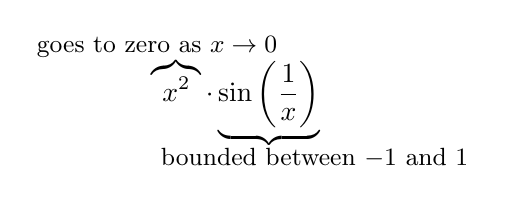
\begin{tikzpicture}
        \node at (0,0) {
          $\overbrace{x^2} \cdot \underbrace{\sin\left(\frac{1}{x}\right)}$
          };
        \node at (-1,.7) {\small{goes to zero as $x\to 0$}};
        \node at (1,-.7) {\small{bounded between $-1$ and $1$}};
      \end{tikzpicture}
    \end{image}
    
    Hence we have
    \[
    x^2 \answer[given]{-1} \le x^2\sin\left(\frac{1}{x}\right) \le x^2 \answer[given]{1}
    \]
    and we see
    \[
    \lim_{x\to 0} x^2 \answer[given]{-1} = \answer[given]{0} = \lim_{x\to 0} x^2 \answer[given]{1}
    \]
    and so by the Squeeze theorem,
    \[
    \lim_{x\to
      0}\left(x^2\sin\left(\frac{1}{x}\right)\right)=\answer[given]{0}.
    \]
  \end{explanation}
\end{example}

\end{document}
